\documentclass[]{article}

% Get better typography
\usepackage[protrusion=true,expansion=true]{microtype}		

% For algorithms
\usepackage[boxruled,linesnumbered,vlined,inoutnumbered]{algorithm2e}
\SetKwInOut{Parameter}{Parameters}
\usepackage[top=2cm, bottom=2cm, left = 1cm, right = 1cm,columnsep=20pt]{geometry}

% For basic math, align, fonts, etc.
\usepackage{amsmath}
\usepackage{amsthm}
\usepackage{amssymb}
\usepackage{mathtools}
\usepackage{mathrsfs}
\usepackage{rotating}
\usepackage{gensymb} % For \degree
\usepackage{booktabs}
\usepackage{graphicx}
\usepackage{float}
\usepackage{xcolor}

\usepackage{enumitem} %for enumerating with letters

\newtheorem{defn}{Definition}[]
\newtheorem{thm}{Theorem}[]
\newtheorem{claim}{Claim}[]
\newtheorem{lemma}{Lemma}[]
\newtheorem{prop}{Property}[]
\newtheorem{ass}{Assumption}[]
\newtheorem{cor}{Corollary}[]

\DeclareMathOperator*{\argmin}{arg\,min}
\DeclareMathOperator*{\argmax}{arg\,max}

\usepackage{courier} % For \texttt{foo} to put foo in Courier (for code / variables)
\usepackage{lipsum} % For dummy text

% For images
\usepackage{graphicx}
\usepackage{subcaption}
\usepackage[space]{grffile} % For spaces in image names

% For bibliography
\usepackage[round]{natbib}

% For color
\usepackage{xcolor}
\definecolor{light-grey}{rgb}{0.95,0.95,0.95}
\definecolor{dark-red}{rgb}{0.4,0.15,0.15}
\definecolor{dark-blue}{rgb}{0,0,0.7}

% For questions and answers
\usepackage[framemethod=tikz]{mdframed}
\newtheorem{question}{Question}
\mdfdefinestyle{que}{
  linecolor=dark-blue,
  backgroundcolor=white!20,
}
\surroundwithmdframed[style=que]{question}
\newtheorem{answer}{Answer}
\mdfdefinestyle{ans}{
  linecolor=dark-red,
  backgroundcolor=white!20
  % , rotatebox
}
\surroundwithmdframed[style=ans]{answer}
\usepackage{environ}
\NewEnviron{Answer}
{%
\noindent
\rotatebox[origin=c]{180}{%
\noindent
\begin{minipage}[t]{\linewidth}
\begin{answer}
\BODY
\end{answer}%
\end{minipage}%
}%
}%

\newif\ifHomeworkOneAnswers
%\HomeworkOneAnswersfalse
\HomeworkOneAnswerstrue

% Only show sections in table of contents and rename
\setcounter{tocdepth}{2}
\renewcommand{\contentsname}{Table of Contents}

% For links (e.g., clicking a reference takes you to the phy)
\usepackage{hyperref}
\hypersetup{
    colorlinks, linkcolor={dark-blue},
    citecolor={dark-blue}, urlcolor={dark-blue}
}

%-------------------------
%	BEGIN DOCUMENT / TITLE
%-------------------------

\begin{document}

%\maketitle
%\hrulefill
%-----------------
%	Homework 1
%-----------------
\newpage
\begin{center}
    \begin{Large}
    CMPSCI 687 Homework 1
    \end{Large}
    \\
    Due September 19, 2019, 11:55pm Eastern Time
\end{center}
\addcontentsline{toc}{subsection}{\textbf{Homework 1}}

\noindent {\bf Instructions: } This homework assignment consists of a written portion and a programming portion. While you may discuss problems with your peers (e.g., to discuss high-level approaches), you must answer the questions on your own. Submissions must be typed (hand written and scanned submissions will not be accepted). You must use \LaTeX. The assignment should be submitted on Gradescope as PDF with marked answers via the Gradescope interface. The source code should be submitted via the Gradescope programming assignment as a .zip file. Include with your source code instructions for how to run your code. You \textbf{must} use Python 3 for your homework code. You may not use any reinforcement learning or machine learning specific libraries in your code, e.g., TensorFlow or PyTorch (you may use libraries like numpy and matplotlib though). The automated system will not accept assignments after 11:55pm on September 19. The tex file for this homework can be found \href{https://people.cs.umass.edu/~pthomas/courses/CMPSCI_687_Fall2019/hw1Source.tex}{here}.


\section*{Part One: Written (63 Points Total)}
\begin{enumerate}
    \item (Your grade will be a zero on this assignment if this question is not answered correctly) Read the class syllabus carefully, including the academic honesty policy. To affirm that you have read the syllabus, type your name as the answer to this problem. 

	{
		\color{blue}
			Ans 1. Aditya Vikram Agarwal
	}

    %
    \item (15 Points) Given an MDP $M=(\mathcal S, \mathcal A, P, d_R, d_0, \gamma)$ and a fixed policy, $\pi$, the probability that the action at time $t=0$ is $a \in \mathcal A$ is:
    \begin{equation}
        \Pr(A_0=a)=\sum_{s \in \mathcal S} d_0(s) \pi(s,a).
    \end{equation}
    Write similar expressions (using only $\mathcal S,\mathcal A,P,R,d_0,\gamma$, and $\pi$) for the following problems.\\
    
    \textbf{Hints and Probability Review:}
    \begin{itemize}
        \item \textbf{Write Probabilities of Events:} In some of the probability hints below that are not specific to RL, we use expressions like $\Pr(a|b)$, where $a$ and $b$ are events.  Remember that in the RL notation used for this class, the values of $\Pr(s_0)$, $\Pr(a_0)$, $\Pr(A_0)$, or $\Pr(A_0 | S_0)$ are all undefined, since those are simply states, actions, or random variables (not events).  Instead, we must write about the probabilities of events.  For example: $\Pr(A_0 = a_0)$ or $\Pr(A_0 = a_0 | S_0 = s_0)$.
        %
        \item \textbf{Bayes' Theorem:} $\Pr(a|b) = \frac{\Pr(b|a) \Pr(a)}{\Pr(b)}$. This is useful for dealing with conditional probabilities $\Pr(a|b)$, where event $a$ occurs before event $b$.  For example, it is often difficult to work with an expression like $\Pr(S_0 = s_0 | A_0 = a_0)$, but much easier to deal with the 3 terms in $\frac{\Pr(A_0 = a_0 | S_0 = s_0) \Pr(S_0 = s_0)}{\Pr(A_0 = a_0)}$.
        %
        \item \textbf{The law of total probability:} For event $a$, and a set of events $\mathcal{B}$,
        $$\Pr(a) = \sum_{b \in \mathcal B} \Pr(b) \Pr(a|b)$$ See the example below for several useful applications of this property.
        \item \textbf{``Extra'' given terms:} Remember that when applying laws of probability, any ``extra'' given terms stay in the result.  For example, applying the law of total probability: $$\Pr(a|c,d) = \sum_{b \in \mathcal B} \Pr(b|c,d) \Pr(a|b,c,d)$$
        %
        \item \textbf{Example problem:} The probability that the state at time $t = 1$ is $s \in \mathcal S$. 
        \begin{align}
        \Pr(S_1 = s) =& \sum_{s_0 \in \mathcal S} \Pr(S_0 = s_0) \Pr(S_1 = s | S_0 = s_0) \\
        %
        =& \sum_{s_0\in \mathcal S} d_0(s_0) \Pr(S_1 = s | S_0 = s_0)\\
        %
        =& \sum_{s_0\in \mathcal S} d_0(s_0) \sum_{a_0\in \mathcal A} \Pr(A_0 = a_0 | S_0 = s_0)\\
        &\times \Pr(S_1 = s | S_0 = s_0, A_0 = a_0)\\
        %
        =& \sum_{s_0\in \mathcal S} d_0(s_0) \sum_{a_0\in \mathcal A} \pi(s_0, a_0) P(s_0, a_0, s).
        \end{align}
    \end{itemize}
    %
    \textbf{Problems:}\\
    \begin{enumerate}[label=\Alph*]
        \item The probability that the action at time $t=3$ is either $ a \in \mathcal A$ or $a' \in \mathcal A$, with $a \ne a'$.
        \\


	{
		\color{blue}
		Ans A.	 \begin{align}
			        \Pr(A_{3} = a \cup A_{3} = a') =& \sum_{s_0 \in \mathcal S} \Pr(S_0 = s_0) \Pr(A_{3} = a \cup A_{3} = a' | S_0 = s_0) \\
				%
				=& \sum_{s_0 \in \mathcal S} d_0(s_0) \sum_{a_0 \in \mathcal A} \Pr(A_0 = a_0 | S_0 = s_0) \Pr(A_{3} = a \cup A_{3} = a' | S_0 = s_0, A_0 = a_0) \\
			        %
			        =& \sum_{s_0 \in \mathcal S} d_0(s_0) \sum_{a_0 \in \mathcal A} \pi(s_0, a_0) \sum_{s_1 \in \mathcal S} \Pr(S_1 = s_1 | S_0 = s_0, A_0 = a_0) \\
				& \times \Pr(A_{3} = a \cup A_{3} = a' | S_0 = s_0, A_0 = a_0, S_1 = s_1) \\
			        %
			        =& \sum_{s_0 \in \mathcal S} d_0(s_0) \sum_{a_0 \in \mathcal A} \pi(s_0, a_0) \sum_{s_1 \in \mathcal S} P(s_0, a_0, s_1) \Pr(A_{3} = a \cup A_{3} = a' | S_1 = s_1) \\
			        %
			        =& \sum_{s_0 \in \mathcal S} d_0(s_0) \sum_{a_0 \in \mathcal A} \pi(s_0, a_0) \sum_{s_1 \in \mathcal S} P(s_0, a_0, s_1) \\
				& \times \sum_{a_1 \in \mathcal A} \Pr(A_1 = a_1 | S_1 = s_1) \Pr(A_{3} = a \cup A_{3} = a' | S_1 = s_1, A_1 = a_1) \\
			        %
			        =& \sum_{s_0 \in \mathcal S} d_0(s_0) \sum_{a_0 \in \mathcal A} \pi(s_0, a_0) \sum_{s_1 \in \mathcal S} P(s_0, a_0, s_1) \sum_{a_1 \in \mathcal A} \pi(s_1, a_1) \\
				& \times \sum_{s_2 \in \mathcal S} \Pr(S_2 = s_2 | S_1 = s_1, A_1 = a_1) \Pr(A_{3} = a \cup A_{3} = a' | S_1 = s_1, A_1 = a_1, S_2 = s_2) \\
			        %
			        =& \sum_{s_0 \in \mathcal S} d_0(s_0) \sum_{a_0 \in \mathcal A} \pi(s_0, a_0) \sum_{s_1 \in \mathcal S} P(s_0, a_0, s_1) \sum_{a_1 \in \mathcal A} \pi(s_1, a_1) \sum_{s_2 \in \mathcal S} P(s_1, a_1, s_2) \\
				& \times \sum_{a_2 \in \mathcal A} \Pr(A_2 = a_2 | S_2 = s_2) \Pr(A_{3} = a \cup A_{3} = a' | S_2 = s_2, A_2 = a_2) \\
			        %
			        =& \sum_{s_0 \in \mathcal S} d_0(s_0) \sum_{a_0 \in \mathcal A} \pi(s_0, a_0) \sum_{s_1 \in \mathcal S} P(s_0, a_0, s_1) \sum_{a_1 \in \mathcal A} \pi(s_1, a_1) \sum_{s_2 \in \mathcal S} P(s_1, a_1, s_2) \\
				& \times \sum_{a_2 \in \mathcal A} \pi(s_2, a_2) \sum_{s_3 \in \mathcal S} \Pr(S_3 = s_3 | S_2 = s_2, A_2 = a_2) \Pr(A_{3} = a \cup A_{3} = a' | S_3 = s_3) \\
			        %
			        =& \sum_{s_0 \in \mathcal S} d_0(s_0) \sum_{a_0 \in \mathcal A} \pi(s_0, a_0) \sum_{s_1 \in \mathcal S} P(s_0, a_0, s_1) \sum_{a_1 \in \mathcal A} \pi(s_1, a_1) \sum_{s_2 \in \mathcal S} P(s_1, a_1, s_2) \\
				& \times \sum_{a_2 \in \mathcal A} \pi(s_2, a_2) \sum_{s_3 \in \mathcal S} P(s_2, a_2, s_3) (\pi(s_{3}, a) + \pi(s_{3}, a')) \\
		        \end{align}
	}
        
        
        \item The expected reward at time $t=6$ given that the action at time $t=5$ is $a \in \mathcal A$ and the state at time $t=4$ is $s\in \mathcal S$.

	{
		\color{blue}
				Ans B. \begin{align}
				\mathbf{E}[R_6 | A_5 = a, S_4 = s] =& \sum_{s_5 \in S} \Pr(S_5 = s_5 | A_5 = a, S_4 = s) \mathbf{E}[R_6 | A_5 = a, S_4 = s, S_5 = s_5] \\
				%
				=& \sum_{s_5 \in S} (\mathbf{E}[R_6 | A_5 = a, S_5 = s_5]) \times \left( \frac{\Pr(S_5 = s_5, A_5 = a | S_4 = s)}{\Pr(A_5 = a | S_4 = s)} \right) \\
				%
				=& \sum_{s_5 \in S} (\sum_{s_6 \in S} \Pr(S_6 = s_6 | A_5 = a, S_5 = s_5) \mathbf{E}[R_6 | A_5 = a, S_5 = s_5, S_6 = s_6]) \times \\
				& \left(  \frac{\Pr(S_5 = s_5, A_5 = a | S_4 = s)}{\Pr(A_5 = a | S_4 = s)} \right)  \\
				%
				=& \sum_{s_5 \in S} (\sum_{s_6 \in S} P( s_5, a, s_6 ) \sum_{a_6 \in A} \Pr(A_6 = a_6 | S_6 = s_6) \mathbf{E}[R_6 | S_6 = s_6, A_6 = a_6]) \times \\
				& \left(  \frac{\Pr(A_5 = a | S_4 = s, S_5 = s_5) \Pr(S_5 = s_5 | S_4 = s)}{ \sum_{s_5 \in S} \Pr(S_5 = s_5 | S_4 = s) \Pr(A_5 = a | S_4 = s, S_5 = s_5)} \right)  \\
				%
				=& \sum_{s_5 \in S} (\sum_{s_6 \in S} P( s_5, a, s_6 ) \sum_{a_6 \in A} \pi(s_6, a_6) R(s_6, a_6)) \times \\
				& \left(  \frac{\pi(s_5, a) \sum_{a_4 \in A} \Pr(A_4 = a_4 | S_4 = s) \Pr(S_5 = s_5 | S_4 = s, A_4 = a_4)}{ \sum_{s_5 \in S} \pi(s_5, a) \sum_{a_4 \in A} \Pr(A_4 = a_4 | S_4 = s) \Pr(S_5 = s_5 | S_4 = s, A_4 = a_4)} \right)  \\
				%
				=& \sum_{s_5 \in S} (\sum_{s_6 \in S} P( s_5, a, s_6 ) \sum_{a_6 \in A} \pi(s_6, a_6) R(s_6, a_6)) \times \\
				& \left(  \frac{\pi(s_5, a) \sum_{a_4 \in A} \pi(s, a_4) P(s, a_4, s_5)}{ \sum_{s_5 \in S} \pi(s_5, a) \sum_{a_4 \in A} \pi(s, a_4) P(s, a_4, s_5)} \right)  \\
				\end{align}
	}
        
        \item The probability that the action at time $t=16$ is $a' \in \mathcal A$ given that the action at time $t=14$ is $a \in \mathcal A$, and the state at time $t=15$ is $s \in \mathcal S$.

	{
		\color{blue}
		Ans C.	 \begin{align}
			        \Pr(A_{16} = a' | A_{14} = a, S_{15} = s) =& \Pr(A_{16} = a' | S_{15} = s) \\
				%
				=& \sum_{a_{15} \in \mathcal A} \Pr(A_{15} = a_{15} | S_{15} = s) \Pr(A_{16} = a' | S_{15} = s, A_{15} = a_{15}) \\
			        %
			        =& \sum_{a_{15} \in \mathcal A} \pi(s, a_{15}) \sum_{s_{16} \in \mathcal S} \Pr(S_{16} = s_{16} | S_{15} = s, A_{15} = a_{15}) \\
				& \times \Pr(A_{16} = a' | S_{15} = s, A_{15} = a_{15}, S_{16} = s_{16}) \\
			        %
			        =& \sum_{a_{15} \in \mathcal A} \pi(s, a_{15}) \sum_{s_{16} \in \mathcal S} P(s, a_{15}, s_{16}) \Pr(A_{16} = a' | S_{16} = s_{16}) \\
			        %
			        =& \sum_{a_{15} \in \mathcal A} \pi(s, a_{15}) \sum_{s_{16} \in \mathcal S} P(s, a_{15}, s_{16}) \pi(s_{16}, a') \\
		        \end{align}
	}
        
        \item The probability that the initial state was $s \in \mathcal S$ given that the action at time $t=1$ is $a' \in \mathcal A$. 

	{
		\color{blue}
		Ans D.	\begin{align}
				\Pr(S_{0} = s | A_{1} = a') =& \frac{\Pr(S_{0} = s) \Pr(A_{1} = a' | S_{0} = s)}{\Pr(A_{1} = a')} \\
			        %
			        =& \frac{d_{0}(s) \sum_{s_{1} \in \mathcal S} \Pr(S_{1} = s_{1} | S_{0} = s) \Pr(A_{1} = a' | S_{0} = s, S_{1} = s_{1})}{\sum_{s_{1} \in \mathcal S} \Pr(S_{1} = s_{1}) \Pr(A_{1} = a' | S_{1} = s_{1})} \\
			        %
			        =& \frac{d_{0}(s) \sum_{s_{1} \in \mathcal S} \Pr(A_{1} = a' | S_{1} = s_{1}) \sum_{a_{0} \in \mathcal A} \Pr(A_{0} = a_{0} | S_{0} = s) \Pr(S_{1} = s_{1} | S_{0} = s, A_{0} = a_{0})}{\sum_{s_{1} \in \mathcal S} \Pr(S_{1} = s_{1}) \pi(s_{1}, a')} \\
			        %
			        =& \frac{d_{0}(s) \sum_{s_{1} \in \mathcal S} \pi(s_{1}, a') \sum_{a_{0} \in \mathcal A} \pi(s, a_{0}) P(s, a_{0}, s_{1})}{\sum_{s_{1} \in \mathcal S} \pi(s_{1}, a') \Pr(S_{1} = s_{1})} \\
			        %
			        =& \frac{d_{0}(s) \sum_{s_{1} \in \mathcal S} \pi(s_{1}, a') \sum_{a_{0} \in \mathcal A} \pi(s, a_{0}) P(s, a_{0}, s_{1})}{\sum_{s_{1} \in \mathcal S} \pi(s_{1}, a') \sum_{s_{0} \in \mathcal S} \Pr(S_{0} = s_{0}) \Pr(S_{1} = s_{1} | S_{0} = s_{0})} \\
			        %
			        =& \frac{d_{0}(s) \sum_{s_{1} \in \mathcal S} \pi(s_{1}, a') \sum_{a_{0} \in \mathcal A} \pi(s, a_{0}) P(s, a_{0}, s_{1})}{\sum_{s_{1} \in \mathcal S} \pi(s_{1}, a') \sum_{s_{0} \in \mathcal S} d_{0}(s_{0}) \sum_{a_{0} \in \mathcal A} \Pr(A_{0} = a_{0} | S_{0} = s_{0}) \Pr(S_{1} = s_{1} | S_{0} = s_{0}, A_{0} = a_{0})} \\
			        %
			        =& \frac{d_{0}(s) \sum_{s_{1} \in \mathcal S} \pi(s_{1}, a') \sum_{a_{0} \in \mathcal A} \pi(s, a_{0}) P(s, a_{0}, s_{1})}{\sum_{s_{1} \in \mathcal S} \pi(s_{1}, a') \sum_{s_{0} \in \mathcal S} d_{0}(s_{0}) \sum_{a_{0} \in \mathcal A} \pi(s_{0}, a_{0}) P(s_{0}, a_{0}, s_{1})} \\
			\end{align}
	}
        
        \item The expected reward at time $t=3$ given that the initial state is $s \in \mathcal S$, the state at time $t=3$ is $s' \in \mathcal S$, and the action at time $t=4$ is $a' \in \mathcal A$.
       
    \end{enumerate}
    
    \item (3 Points) In 687-Gridworld, if we changed how rewards are generated so that hitting a wall (i.e., when the agent would enter an obstacle state, and is placed back where it started) results in a reward of $-10$, then what is $\mathbf{E}[R_t|S_t=17,A_t=\text{AL}, S_{t+1}=17]$?
    \\
	
	{
		\color{blue}
		Ans 3. \begin{align}
		            \mathbf{E}[R_t|S_t=17,A_t=\text{AL}, S_{t+1}=17] =& \sum_{r \in R_t} r \times \Pr(R_t=r|S_t=17,A_t=\text{AL},S_{t+1}=17) \\
		            %
		            =& -10 \times \Pr(R_t=-10|S_t=17,A_t=\text{AL},S_{t+1}=17) \\
			& + 0 \times  \Pr(R_t=0|S_t=17,A_t=\text{AL},S_{t+1}=17)\\
			%
		           =& -10 \times \frac{\Pr(R_t=-10,S_{t+1}=17|S_t=17,A_t=\text{AL})}{\Pr(S_{t+1}=17|S_t=17,A_t=\text{AL})}\\
		            %
		            =& -10 \times \frac{0.8}{0.8+0.1}\\
		            %
		            =& -\frac{8}{0.9}.
		        \end{align}
		        Therefore,
		        \begin{equation}
		            \mathbf{E}[R_t|S_t=17,A_t=\text{AL}, S_{t+1}=17]=-\frac{8}{0.9}.
		        \end{equation}
	}

	
    
    \item (2 Points) How many deterministic policies are there for an MDP with $|\mathcal S|< \infty$ and $|\mathcal A|<\infty$? (You may write your answer in terms of $|\mathcal S|$ and $|\mathcal A|$).

	{
		\color{blue}
			Ans 4. For an MDP with $|\mathcal S|< \infty$ and $|\mathcal A|<\infty$, the number of deterministic policies is $|\mathcal S| \times |\mathcal A|$.
			\\
			Explanation: For a policy to be deterministic, $\pi(s, a) \in \{0, 1\}$ $\forall s \in \mathcal S$, $a \in \mathcal A$. As each row in the deterministic policy table (each row corresponds to a state) can now have only one entry as 1 and all other entries as 0, the possible number of permutations for that row is $|\mathcal A|$. This is done for all rows of the deterministic policy table. As there are $|\mathcal S|$ rows in the deterministic policy table, the total number of combinations for the deterministic policy table is $|\mathcal S| \times |\mathcal A|$. Therefore, there are $|\mathcal S| \times |\mathcal A|$ number of deterministic policies for an MDP with $|\mathcal S|< \infty$ and $|\mathcal A|<\infty$.
	}
    
    
    \item (5 Points) Give an example of an MDP with $|\mathcal S| < \infty, |\mathcal A| = \infty$, and $\gamma < 1$ such that an optimal policy \emph{does not} exist. Give an example of an MDP with $|\mathcal S| = \infty, |\mathcal A| < \infty$, and $\gamma < 1$ such that an optimal policy exists.

	{
		\color{blue}
			Ans 5. Consider an MDP with an inital state $s_0$ that transitions to $s_\infty$ with a probability of 0.5 for any action taken and stays at $s_0$ with probability of 0.5 for any action taken. In this case, our action set is $\mathcal A$ = [0, 5). Gamma is set to 0.9. Rewards given to the agent for taking action $a \in \mathcal A$ in state $s_0$  are such that the reward function $R_t$ = a for $0 \leq a < 1$, $R_t$ = a - 1 for $1 \leq a < 2$, and $R_t = 0$ for $a \geq 2$ . In this case, we do not have a particular maximum value that the reward can be. This is because at any timestep there exists another action which if taken yields a better reward than any action we choose that generates a certain reward at that timestep. In other words, at any time step, and for whatever action we chose in order to maximize the reward (and consequently the total return), we are certain that there exists another action that yields a better reward (and consequently a better total return) at that timestep. For example, if we were to take an action $a = 0.9999$ that generates a reward of 0.9999, there would still exist another possible action, say $a' = 0.99999999$, which if taken would have generated a reward of 0.99999999.  This would be true for any action $a \in \mathcal A$ that yields a reward r corresponding to that action, that there always exists some $a' \in \mathcal A$ such that the reward obtain by taking action a' in state s would yield a reward r' that is better than the reward r yielded by taking action a at that state s at that timestep t. Thus, there would always be some action a' with reward r' such that $r' > r$ where r is the reward obtained by taking action $a \in \mathcal A$ and $a \ne a'$ . Therefore, we would not be able to find the best reward that the agent can obtain at any time step and consequently we cannot find a policy that yields the maximum expected sum of discounted rewards. Therefore, arg max J($\pi$) is an empty set. So, this is an example of an MDP with $|\mathcal S| < \infty$, $|\mathcal A| = \infty$, and $\gamma < 1$ in which an optimal policy does not exist. \\
			The Mountain Car problem with $\gamma$ = 0.5 is a nice example of an MDP with $|\mathcal S| = \infty$, $|\mathcal A| < \infty$, and $\gamma < 1$ in which an optimal policy exists.
	}
    
    \item (3 Points) Read about the Pendulum domain, described in Section 5.1 of \href{https://homes.cs.washington.edu/~todorov/courses/amath579/reading/Continuous.pdf}{this} paper (Reinforcement Learning in Continuous Time and Space by Kenji Doya). Consider a variant where the initial state has the pendulum hanging down with zero angular velocity always (a deterministic initial state where the pendulum is hanging straight down with no velocity) and a variant where the initial angle is chosen uniformly randomly in $[-\pi,\pi]$ and the initial velocity is zero. Which variant do you expect an agent to require more episodes to solve? Why? Note: We did not talk about the complexity of solving MDPs in class yet---we want you to provide your best guess here.

	{
		\color{blue}
			Ans 6. I expect the agent to require more episodes to solve in the variant in which the initial state has the pendulum hanging down with zero angular velocity always than the variant in which the initial angle of the pendulum is chosen uniformly randomly in [- $\pi$, $\pi$] and the initial velocity is zero. This is because if the agent always starts straight down with zero angular velocity, then it would require to swing back and forth for a while in order to accumulate the angular velocity that would be enough for it to reach the very top and sway there to balance itself around the very top. In this case, a lot of time steps are wasted in order to build that momentum required to bring the pendulum at the very top. It would happen in a lot of episodes that due to that wastage of time, before the pendulum reaches the very top and balances itself, the episode would have been finished (t = 20 would have been reached) or even if the episode did not finish before the pendulum reached the very top, it would have reached the very top very late and would have not acquired a high return. Note that by very top I mean that $|\theta| < \frac{\pi}{4}$. However, if it starts at some angle already, then by the time it reaches the straight bottom position, it would already have acquired some angular momentum. This would only take a few time steps (only from the start time to the time it falls to the straight down position), in contrast to the variant in which the pendulum started with zero angular momentum straight down (as it would waste a lot of time as it would need to sway back and forth to build the required angular momentum). Therefore, when in a few time steps the latter variant would have reached the very bottom having built some angular momentum already, it could quickly reach the top position, and there would be many episodes in which the pendulum reaches the very top and balances itself before the episode finishes and a lot more return would be obtained. Additionally, in this latter variant the pendulum would have explored many states on its way down already, and really quickly, so it would have a rough idea about what actions are to be taken in those states to reach the top quickly. So, I expect the agent to require more episodes to solve in the variant in which the initial state has the pendulum hanging down with zero angular velocity always than the variant in which the initial angle of the pendulum is chosen uniformly randomly in [- $\pi$, $\pi$] and the initial velocity is zero.
	}
    
    \item (1 Point)  How many episodes do you expect an agent should need in order to find near-optimal policies for the gridworld and pendulum domains? 
    %
    Note: We did not talk about the complexity of solving MDPs in class yet---we want you to provide your best guess here. 
    \\

	{
		\color{blue}
			Ans 7. I expect 279,841 to be the number of episodes an agent would need in order to find the near-optimal policies for the gridworld domain. This is because the gridworld has 23 states and 4 actions that it can taken at each state. So, if the agent is at any state and can take 4 actions at that state. Therefore, the number of episodes in which it should reach the near optimal policies would be $23^4$ which is 279,841. \\
			I expect 400 to be the number of episodes an agent would need in order to find the near-optimal policies for the pendulum domain. This is because the pendulum has only two directions of movement possible (clockwise or anti-clockwise), and the episode ends when $t = 20$. So, it should be about $20^2$ episodes which is 400 episodes that the agent should take to reach the near optimal policies.
	}
    
    \item (5 Points) Select a problem that we have not talked about in class, where the agent does not make Markovian observations about the world around it. Describe how the environment for this problem can be formulated as an MDP by specifying $(\mathcal S, \mathcal A, P, [d_r\text{ or } R], d_0, \gamma)$ (your specifications of these terms may use English rather than math, but be precise). 

	{
		\color{blue}
			Ans 8. Consider the task in which an agent tries to play a musical piece on a piano. In this case, the state set contains all the key notes of the piano including the state in which no key is played (blank key note is considered as a state called blank state). The actions correspond to the actuators moving the arms of the agent in order to reach a particular key and the actuators moving the fingers to press/release a key. So, the action set is \{Attempt Moving Left Arm Towards Left, Attempt Moving Left Arm Towards Right, Attempt Moving Right Arm Towards Right, Attempt Moving Right Arm Towards Left, Attempt Left Arm Stay Still, Attempt Right Arm Stay Still, Attempt Pressing Left Finger 1, Attempt Pressing Left Finger 2, Attempt Pressing Left Finger 3, Attempt Pressing Left Finger 4, Attempt Pressing Left Finger 5, Attempt Pressing Right Finger 1, Attempt Pressing Right Finger 2, Attempt Pressing Right Finger 3, Attempt Pressing Right Finger 4, Attempt Pressing Right Finger 5, Attempt Releasing Left Finger 1, Attempt Releasing Left Finger 2, Attempt Releasing Left Finger 3, Attempt Releasing Left Finger 4, Attempt Releasing Left Finger 5, Attempt Releasing Right Finger 1, Attempt Releasing Right Finger 2, Attempt Releasing Right Finger 3, Attempt Releasing Right Finger 4, Attempt Releasing Right Finger 5\}. The reward given is +1 if a correct note is played and -1 if a wrong note is played. Force sensors in fingers are used to know if the fingers are pressed or released. Motion sensors are used to know the direction and distance the arms were moved. Although, the agent has no sound sensors to know the sounds of the notes it plays. The reward discount parameter, $\gamma$ = 1. The initial state is the state in which no key is pressed (blank state). So, at time $t$, at the current key note, a particular action (moving arms or moving fingers to press/release the keys) taken at time $t$ results to transitioning to the next state (next key note). As the agent does not have any sound sensor, it essentially cannot precisely measure its true state. This is because the agent would not be able to determine which key it has pressed. For example, the agent attempts to press Left Finger 1 and it stochastically pressed Left Finger 3. Due to the absence of sound sensors, it would not be able to precisely meassure the state. Thus, the agent will not fully observe the states.
	}
    \\
    
    \item (5 Points) We refer to the discounted sum of rewards, $\sum_{t=0}^\infty \gamma^t R_t$, as the \emph{return}. Let an MDP exist such that it has two optimal policies. Can the expected value of their returns differ? If so, give an example. If not, explain why. Can the variance of their returns differ? If so, give an example. If not, explain why.

	{
		\color{blue}
			Ans 9. No. the expected values of return of two optimal policies of an MDP cannot differ. This is because the optimal policy of an MDP is definded as $\pi^* \in arg max J(\pi) \forall \pi \in \mathcal \pi$, so an optimal policy essentially has the highest expected return among all the policies of that MDP. If the expected values of the optimal policies differ, then one of the optimal policies would have a lesser expected value of return than the other optimal policy. This would mean that the optimal policy having lesser expected value of return would not remain optimal anymore. The difinition of optimal policy requires that there be no other policy of which the expected value of return be higher than the optimal policy. Therefore, all optimal policies of the MDP must have equal expected values of return. \\
		Yes, the expected values of their variance can differ. Consider an MDP with an initial state $s_0$ and another state $s_\infty$. There are two actions, $a_0$ and $a_1$, and both actions transition from $s_0$ to $s_\infty$ with probabilities of 0.5 and from $s_0$ to  $s_0$ with probabilities of 0.5. The reward for action $a_0$ is drawn from the uniform distribution on [0, 1] (variance $\frac{1}{12}$) and the reward for action $a_1$ is drawn from the normal distribution $\mathcal N(0.5, 1)$. If one optimal policy (say $\pi^*_1$) could have $\pi^*_1(s_0, a_0) = 0.7$ and $\pi^*_1(s_0, a_1) = 0.3$ while another optimal policy (say $\pi^*_2$) has $\pi^*_2(s_0, a_0) = 0.3$ and $\pi^*_2(s_0, a_1) = 0.7$. Both policies are optimal as they have equal expected values of their returns, although the vairances of their returns differ.
	}
    
    \item (2 Points) Consider the one state MDP where in $s_0$ there are three actions, $a_0$, $a_1$, $a_2$, and all actions transition to $s_\infty$ with probability $0.5$ and stay in $s_0$ otherwise. The reward for taking actions $a_0$, $a_1$ are drawn from the uniform distribution on $[0,1]$ and the normal distribution $\mathcal{N}(0.5,1)$, respectively. The reward for $a_3$ is always $0.25$. What are all the optimal policies of this MDP? 

	{
		\color{blue}
			Ans 10. The mean of the uniform distribution on [0, 1] is (1 - 0) / 2 which is 0.5. The mean of the normal distribution $\mathcal N(0.5, 1)$ is 0.5. As the mean of a distribution represents the expected value for the random variable having that distribution, therefore the expected values of the rewards that the agent receives by taking action $a_0$ and $a_1$ in state $s_0$ are 0.5 and 0.5 respectively. However, the expected value of the reward that the agent receives by taking action $a_2$ in state $s_0$ is only 0.25. So, all the optimal policies for this MDP are the ones for which: \\
	$\pi^*(s_0, a_0) = p1$, $\pi^*(s_0, a_1) = p2$, $\pi^*(s_0, a_2) = 0$, $\forall p1 \in \mathbb{R}$, $p1 \geq 0, p2 \geq 0$, and $p1 + p2 = 1$

	}
    
    %
    \item (2 Points) Read the Wikipedia page on \href{https://en.wikipedia.org/wiki/Markov_chain}{Markov chains}. A state in a \emph{Markov chain} is \emph{irreducible} if it is possible to get to any state from any state. An MDP is \emph{irreducible} if the Markov chain associated with every deterministic policy is irreducible. A state in a \emph{Markov chain} has \emph{period} $k$ if every return to the state must occur in multiples of $k$ time steps. More formally,
    $$
    k=\operatorname{gcd}\{t>0: \Pr (S_t=s|S_0=s)>0\}.
    $$
    %
    A Markov chain is \emph{aperiodic} if the period of every state is $k=1$. Can an MDP be aperiodic and \emph{not} irreducible? If so, give an example. If not, explain your reasoning. 

	{
		\color{blue}
			Ans 11. Yes, an MDP can be aperiodic and not irreducible. Consider an MDP that has only two states, $s$ and $s'$. There is only one action, $a$, in the action set. $s$ transitions to $s$ with probability 0.5 when action $a$ is taken, $s$ transitions to $s'$ with probability 0.5 when action $a$ is taken, and $s'$ transitions to $s'$ with probability 1 when action $a$ is taken. Consider $\gamma = 1$ and rewards as 1 always. The initial state is $s$ always. This MDP is aperiodic, as both states, $s$ and $s'$, have non-zero probabilities to be reached for each $t \geq 1$. Therefore, the MDP is aperiodic. Additionally, the MDP is not irreducible as we cannot reach from state $s'$ to $s$. In other words, the probability of reaching from $s'$ to $s$ is 0. Therefore, this is an example of an MDP which is aperiodic  and not irreducible.
	}
			
    
   
    \item (5 Points) The state of a Markov chain is \emph{positive recurrent} if the expected time until the state recurs is finite. A Markov chain is \emph{positive recurrent} if all states are positive recurrent. Give an example of an MDP with $|S|>2$ states that is positive recurrent and aperiodic. For any number of states $|S|$, can you think of a simple way of defining state transitions such that the MDP is positive recurrent and aperiodic? Explain your methodology (a picture might be useful). 

	{
		\color{blue}
			Ans 12. Consider an MDP with states $s_0$, $s_1$, and $s_2$. The action set contains only one action, $a$. Consider $\gamma$ = 1. Consider the initial state as $s_0$. The rewards are +1 always. $s_0$ transitions to $s_1$ with probability 0.5 when action $a$ is taken, $s_0$ transitions to $s_0$ with probability 0.5 when action $a$ is taken, $s_1$ transitions to $s_2$ with probability 1 when action $a$ is taken, and $s_2$ transitions to $s_0$ with probability 1 when action $a$ is taken. This is an MDP with $|\mathcal S| > 2$, and that is positive recurrent (expected time until each state is reached is finite) and aperiodic (period of each state is 1). \\
		For any number of states $|\mathcal S|$, if we have the transition function such that the MDP is irreducible (an MDP is irreducible if the markov chain associated with every deterministic policy is irreducible), and if at least one state of the MDP is such that it is involved in $n$ cyclic loops with other states where either $n \geq 2$ and at least one pair of cycles have co-prime number of transition edges, or if at least one state of the MDP has a transition edge to itself. Note that a transition edge exists only if the probability of that transition is non-zero. Irreducible MDPs make them positive recurrent, as every state can reach any state so the expected time until each state recurs is finite. Additionally, to make any MDP with $|\mathcal S|$ states aperiodic, if atleast one state has a self loop, then the period of that state is 1 and the periods of other states are also 1 because when other states transition to the state with the self loop, then from there onwards 1, 2, ... loop transitions can take place. Also, the MDP would be aperiodic if at least one state is involved in more than 2 cycles and if at least one pair of those cycles have a co-prime number of edges. This is because once the transition from state comes to this state involved in cycles with at least co-prime number of edges, then there is no pattern in the time steps that the original state is being reached. (See example figure below)

		\begin{figure}[H]
		    \centering
		    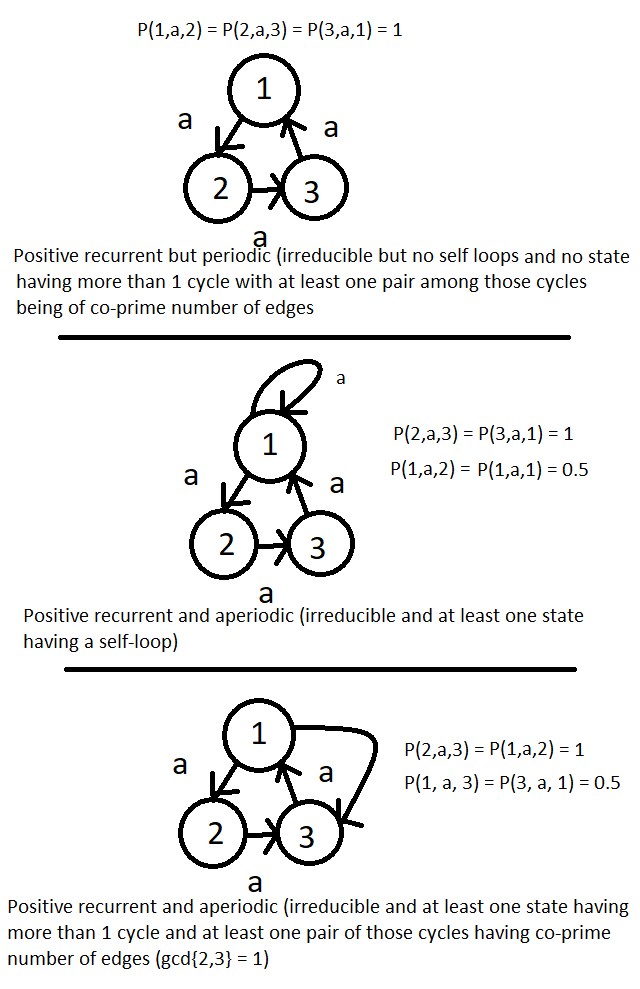
\includegraphics[width=0.6\textwidth]{loop.png}
		    \caption{Answer 12 figure}
		    \label{fig: Answer 12 figure}
		\end{figure}
	}
    
   
    
    \item (1 point) Let a tabular policy representation be used to represent stochastic policies for an MDP with $n$ states and $m$ actions. What is the sum of every element in the matrix representation of this policy? Why?

	{
		\color{blue}
		Ans 13. The sum of every element in the tabular policy representation for an MDP with n states and m actions is n.
		\\
		Explanation: If we consider the $s_i^{th}$ row in the tabular representation of the policy, where $s_i \in \mathcal S$, then the sum of all elements in this row is 1. This is done for all rows of the tabular policy table. As there are n rows (n states), the total sum of all elements in all the rows would be $1 \times n$ which is n. Therefore, the sum of every element in the tabular policy representation for an MDP with n states and m actions is n.
	}
   
    
    \item (2 Points) Describe a real-world problem and how it can be reasonably modeled as an MDP where $R_t$ is \emph{not} a deterministic function of $S_t, A_t,$ and $S_{t+1}$, and is not a bandit problem. 

	{
		\color{blue}
			Ans 14. Consider a tutoring system in which the motive of the agent is to maximize the total test score of the student over 10 tests, one per day after the student after the student has been taught that day. The states of the MDP are the days (1 to 10 natural numbers) and an $s_{\infty}$. The actions of the agent are to teach the chapters to the student anywhere between 1 - 2 hours per day. Consider $\gamma = 1$. The initial state is day 1. The reward +1 if the student recevies 100/100 on a test, and the reward is 0 otherwise. The transition function is such that for any day (state), the agent teaches the student 1 - 2 hours that day (action), then the MDP transitions to the next day (next state). The reward generated for each day is after the student has been taught that day (after that day's test has been taken). In this example, $R_t$ is certainly not a deterministic function of $S_t$, $A_t$, and $S_{t + 1}$. Also, day 10 (state 10) transitions to $s_{\infty}$. This is because we cannot with 100\% certainty say that on any particular day if the agent teaches the student anywhere between 1 - 2 hours that day then the student would receive 100/100 score on the test (+1 reward) or not (0 reward). This is because the test might be extremely difficult or extremely easy for what the agent had taught the student that day. Additionally, this is not a bandit problem either, as there are 10 states (10 days) and an $s_\infty$. Therefore, this is a real-world example in which $R_t$ is not a deterministic function of $S_t$, $A_t$, and $S_{t + 1}$ and it is not a bandit problem.
	}
    
    
    \item (2 Points) If you know $(\mathcal S, \mathcal A, P, R, d_0, \gamma)$, can you derive $d_R$? Prove your answer is correct. 

	{
		\color{blue}
			Ans 15. No, if we know $(\mathcal S, \mathcal A, P, R, d_0, \gamma)$, we cannot derive $d_R$. This is because $d_R$ is the conditional distribution over $R_t$ given $S_t$, $A_t$, and $S_{t+1}$, whereas $R$ is just the expected value (mean) of $R_t$ given $S_t$ and $A_t$. There can be many distributions having the same expected value (mean). So, just knowing the mean would not guarantee that we know it is coming from a particular distribution. For example, the expected value could be 0.5 but it could be coming from a uniform distribution over [0, 1] or a normal distribution $N(0.5, 1)$. So, this is an example where the reward function can have different $d_R$. This shows that if we know $(\mathcal S, \mathcal A, P, R, d_0, \gamma)$, we cannot derive $d_R$.
	}
    
    \item (2 Points) If you know $(\mathcal S, \mathcal A, P, d_R, d_0, \gamma)$, can you derive $R$? Prove your answer is correct. 

	{
		\color{blue}
		Ans 16. Yes, if we know $(\mathcal S, \mathcal A, P, d_R, d_0, \gamma)$, we can derive $R$.
			\begin{align}
		            R(s,a) =& \mathbf{E}[R_t|S_t=s,A_t=a] \\
		            %
		            =& \sum_{s' \in \mathcal S} \Pr(S_{t+1}=s'|S_t=s,A_t=a) \mathbf{E}[R_t|S_t=s,A_t=a, S_{t + 1} = s'] \\
		            %
		            =& \sum_{s' \in \mathcal S} P(s,a,s') \sum_{r \in R_t} r \times \Pr[R_t = r|S_t=s,A_t=a, S_{t + 1} = s'] \\
		        \end{align}
			\begin{flushright}
							(as $d_R$ is the Conditional Distribution over $R_t$ given $S_t$ = s, $A_t$ = a, $S_{t + 1}$ = s')
			\end{flushright}
			As we know P, $d_R$, and $r \in \mathcal R$ (we know r as $d_R$ is the Conditional Distribution which is known over $R_t$) we can derive $\mathbf{E}[R_t|S_t=s,A_t=a]$ which is $R(s, a)$. Therefore, if we know $(\mathcal S, \mathcal A, P, d_R, d_0, \gamma)$, we can derive $R$.
	}
    
    \item (2 Points) Describe a real-world problem and how it can be reasonably modeled as an MDP where $R_t$ is a deterministic function of $S_t$.

	{
		\color{blue}
			Ans 17. Consider the task of an agent rowing a boat in a river in which the motive of the agent is to cross the river and reach any point at the edge of the opposite shore. In this  problem, the state set contains all the positions in the river and all the positions on the edges of both the shores. The action set contains attempts of all possible movements of the boat, in each direction (360\degree around). The initial state is at the edge of one shore at a particular point. Consider $\gamma = 1$. Taking an action (attempting to move along a direction) at a state (position in the river) leads to transitioning to another state (position in the river). In this case, we define $R_{t}$ to be +1 if $S_{t}$ is a state in which the agent is  considered to have reached any point at the edge of the opposite shore of the river and $R_{t}$ to be 0 if $S_{t}$ is a state in which the agent is considered to be at every other position. Therefore, this is an example of an MDP in which $R_{t}$ is a deterministic function of $S_{t}$.
	}
    
    \item (2 Points) Describe a real-world problem and how it can be reasonably modeled as an MDP where the reward function, $R$, would \emph{not} be known. 

	{
		\color{blue}
			Ans 18. Consider the task of an agent rowing a boat in a river in which the motive of the agent is to cross the river and reach any point at the edge of the opposite shore. In this  problem, the state set contains all the positions in the river and all the positions on the edges of both the shores. The action set contains attempts of all possible movements of the boat, in each direction (360\degree around). The initial state is at the edge of one shore at a particular point. Consider $\gamma = 0.5$. +1 reward is obtained by the agent if the agent reaches one step closer to the edge of the opposite shore of the river and -1 if agent reaches one step away from the edge of the other shore (in other words, -1 reward is obtained if the agent reaches one step closer to the edge of the current shore). Here, at any time step, the distance from the agent to the shore is the perpendicular distance from the agent to the edge of that shore. In this case, we do not know the transition function due to the complex dynamics of the water currents in the river. The flow of water in the river is so unpredictable and complex  that we do not know the probability of reaching a particular point (the next state)  if we attempt to move along a particular direction (action at time t) when we are at a particular state (particular position in the river) at time t. The transition function is also non-deterministic, as $P(s, a, s')$ can be any value such as 0.3231, etc. Neither do we know the reward function, $R$, as we just do not know the expected reward the agent would get at time t, if it selected an action from the action set (attempting to move in a direction which could be any direction 360 degrees around) when it is at a given state (point in the river) at time t. For example, we might attempt moving at a certain angle that should have taken us closert to the edge of the opposite shore if the river were perfectly still, but the complex dynamics of the ocean current unpredicatbly takes us at a position along some other direction that takes us one step away from the edge of the opposition shore. Although the rewards, +1 and -1, do exist, we just do not know what the expected reward the agent could receive is, as we just do not know the distribution over whether we would reach one step closer to the opposite shore or one step closer to the edge of the shore we started at, from the current position and taking an action at time t. We therefore do not know the reward function, $R$, and only know what reward (+1 or -1) is obtained once the action is taken. Therefore, this is an example of an MDP in which the reward function $R$ is not known.
	}


    
    
    \item (2 Points) Describe a real-world problem and how it can be reasonably modeled as an MDP where the transition function, $P$, would be known.

	{
		\color{blue}
			Ans 19. Consider the task in which an agent tries to play a musical piece on a piano. In this case, the state set contains all the key notes of the piano including the state in which no key is played (blank key note is considered as a state called blank state). The actions correspond to the actuators moving the arms of the agent in order to reach a particular key and the actuators moving the fingers to press/release a key at a certain position. So, the action set is \{Attempt Moving Left Arm Towards Left, Attempt Moving Left Arm Towards Right, Attempt Moving Right Arm Towards Right, Attempt Moving Right Arm Towards Left, Attempt Left Arm Stay Still, Attempt Right Arm Stay Still, Attempt Pressing Left Finger 1, Attempt Pressing Left Finger 2, Attempt Pressing Left Finger 3, Attempt Pressing Left Finger 4, Attempt Pressing Left Finger 5, Attempt Pressing Right Finger 1, Attempt Pressing Right Finger 2, Attempt Pressing Right Finger 3, Attempt Pressing Right Finger 4, Attempt Pressing Right Finger 5, Attempt Releasing Left Finger 1, Attempt Releasing Left Finger 2, Attempt Releasing Left Finger 3, Attempt Releasing Left Finger 4, Attempt Releasing Left Finger 5, Attempt Releasing Right Finger 1, Attempt Releasing Right Finger 2, Attempt Releasing Right Finger 3, Attempt Releasing Right Finger 4, Attempt Releasing Right Finger 5\}. The reward given is +1 if a correct note is played and -1 if a wrong note is played. Sound sensors in the agent are used to know if the note producing a sound is the correct node or not, thereby the rewards are generated. Force sensors in the fingers are used to know if the fingers are pressed or released. Motion sensors are used to know the direction and distance the arms were moved. The reward discount parameter, $\gamma$ = 1. The initial state is the state in which no key is pressed (blank state). So, at time $t$, at the current key note, a particular action (moving arms or moving fingers to press/release the keys) taken at time $t$ results to transitioning to the next state (next key note) with some probability. In this problem, given a current state (current key note) at time $t$ and the action taken by the agent (moving the hands or fingers) at time $t$, we essentially know the probability of the next key note (next state). In fact, the transition function is deterministic in this example, as we know with certainty what the next note (next state) would be. For example, if our current note were a blank note and we just attempt pressing right finger 5, then we are guaranteed that the next state would be the note at the position just beneath the right finger 5. This is because there are no obstacles in the environment preventing the motion of the arm or finger and the actuators are really good such that when it attemps an action then that action happens with a probability of 1. In other words, each action has probability 1 of occurence in practice if that action is chosen at a given state.  Therefore, this is an example of an MDP in which the transition function $P$ is known.
	}
    
    \item (2 Points) Describe a real-world problem and how it can be reasonably modeled as an MDP where the transition function, $P$, would \emph{not} be known.

	{
		\color{blue}
			Ans 20. Consider the task of an agent rowing a boat in a river in which the motive of the agent is to cross the river and reach the edge of the opposite shore, possibly at the exact opposite point on the edge of the other shore. In this  problem, the state set contains all the positions  in the river and at the positions of the edges of both the shores. The action set contains attempts of all possible movements of the boat, in each direction (360\degree around). The initial state is at the edge of one shore at a particular point. Consider $\gamma = 0.5$. +10 reward is obtained by the agent if the exact opposite point on the edge of the other shore of the river is reached, -1 if any other point on the edge of the other shore is reached, and -10 if it reaches any point of the edge of the current shore. In this case, we do not know the transition function due to the complex dynamics of the water currents in the river. The flow of water in the river is so unpredictable and complex  that we do not know the probability of reaching a particular point (the next state)  if we attempt to move along a particular direction (action at time t) when we are at a particular state (particular position in the river) at time t. We would need to know details such as the velocities of each molecule of water, frictional force at each point of contact of the boat and the river, etc in order to know the probabilities of reaching the next state given current state and current action. It  is very complex to model the dynamics of the water flowing through the river and due to such complexity, we do not know the transition function. Therefore, this is an example of an MDP in which the transition function $P$ is not known.
	}
    
\end{enumerate}

\section*{Part Two: Programming (25 Points Total)}

\noindent\textbf{More-Watery 687-Gridworld.} For this assignment, we will be working with a slightly modified version of the 687-Gridworld domain described in class and in the class notes. In this new Gridworld, called More-Watery Gridworld, there are two extra water states located in state 7 and state 17, as shown in Figure \ref{fig: watery gridworld}. Implement More-Watery Gridworld. 

\textbf{Codebase.} We have provided a template for programming the homework on the github repository for this class located  \href{https://github.com/bmetevier/rl-framework-687-public}{here}. You do \emph{not} need to use this template for the assignment. After the due date for this assignment, an example will be posted on this site. 

\begin{figure}[h!!!]
    \centering
	[Image omitted]
    %\includegraphics[width=1\textwidth]{watery_gridworld.pdf}
    \caption{A more watery version of 687-Gridworld. Water states are located in state 7, state 17, and state 21.}
    \label{fig: watery gridworld}
\end{figure}

\begin{enumerate}[label=\Alph*]
    \item (5 Points) Have the agent uniformly randomly select actions. Run $10,\!000$ episodes. Report the mean, standard deviation, maximum, and minimum of the observed discounted returns. 

	{
		\color{blue}
			Ans A. Mean: -9.161382 \\
				Standard Deviation: 7.304394 \\
				Maximum: 4.782969 \\
				Minimum: -45.245360 \\
	}
    
    \item (5 Points) Find an optimal policy (you may do this any way you choose, including by reasoning through the problem yourself). Report the optimal policy here. Comment on whether it is unique.

	{
		\color{blue}
			Ans B. One of the optimal policies is:
	
		\begin{align}
		        \begin{bmatrix}
		        right&    right&    right&    right&     down     \\
		    up&    right&    right&    right&     down     \\
		    up&       down&       XXXXX&    right&     down     \\
		    up&       left&       XXXXX&    right&     down \\
		    up&       left&       right&    right&    right\\
		        \end{bmatrix}
	    \end{align}

		However, the optimal policy is not unique. Yet another optimal policy is:

		
		\begin{align}
		        \begin{bmatrix}
		        right&    right&    right&    right&     down     \\
		    up&    right&    right&    right&     down     \\
		    up&       down&       XXXXX&    right&     down     \\
		    up&       left&       XXXXX&    right&     down \\
		    up&       left&       right&    right&    down\\
		        \end{bmatrix}
	    \end{align}
	}

    \item (5 Points) Run the optimal policy that you found in the previous question for $10,\!000$ episodes. Report the mean, standard deviation, maximum, and minimum of the observed discounted returns.

	{
		\color{blue}
			Ans C. Mean: 2.987287 \\
				Standard Deviation: 2.922822 \\
				Maximum: 4.782969 \\
				Minimum: -34.031605 \\
	}

    \item (5 Points) The distribution of returns is often not normal, thus it cannot be fully characterized by its mean and standard deviation. To provide more information about the performance, the empirical distribution of returns can be reported.
    
    For a random variable, $X$, its \textit{cumulative distribution function} (CDF), $F_X$, is defined as $F_X(x) \coloneqq \Pr(X \le x)$. The empirical CDF, $\hat F$, for a sequence of $n$ samples of $X$, $X_1,\dotsc,X_n$ is given by the function
    %
    \begin{equation*}
        \hat F_n(x) \coloneqq \frac{1}{n} \sum_{i=1}^n \mathbf{1}_{X_i \le x},
    \end{equation*}
    %
    where $X_i$ is the $i^\text{th}$ sample of $X$ and $\mathbf{1}_A$ is the indicator function of an event $A$, i.e., $\mathbf{1}_A=1$ if $A$ is true and $0$ otherwise. 
    
    The quantile function, also referred to as the inverse CDF, is the function $Q(\tau) \coloneqq \inf \{ x \in \mathbb{R} \colon \tau \le F_X(x) \}$ for $\tau \in (0,1)$. The empirical quantile function, $\hat Q$, can be constructed by considering the order statistics, $Z_i$, the sorted samples of $X_i$ such that $Z_1 \le Z_2 \le \dotsc \le Z_n$. The empirical quantile function is given by
    %
    \begin{equation*}
        \hat Q(\tau) \coloneqq Z_{\lfloor (n+1)\tau \rfloor}.
    \end{equation*}
    %
    Both the CDF and quantile functions capture all the information about a random variable, but for plotting purposes the quantile function is often preferred. This is because we are interested in maximizing returns, so the quantile function has a more natural interpretation as higher is better. 
    
    Plot the distribution of returns for both the random policy and the optimal policy using $10,\!000$ trials each. You must clearly label each line and axis. Additionally, report the random seed used for the experiments. 

	{
		\color{blue}
		Ans D. The random seeds used for the experiments is 687.
		
		\begin{figure}[H]
		    \centering
		    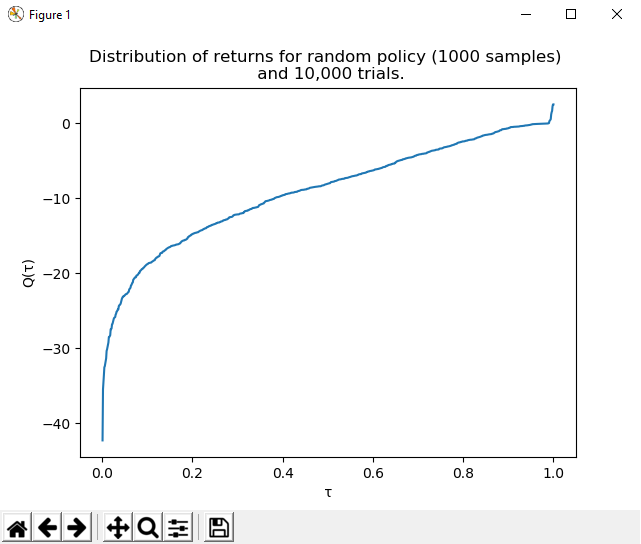
\includegraphics[width=0.6\textwidth]{watery_2.png}
		    \caption{Distribution of returns for the random policy (1000 samples) using 10,000 trials.}
		    \label{fig: watery gridworld distribution policy}
		\end{figure}
		
			
		\begin{figure}[H]
		    \centering
		    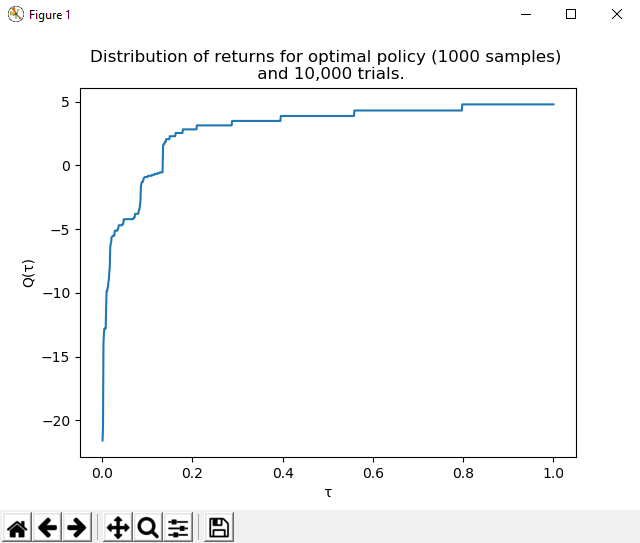
\includegraphics[width=0.6\textwidth]{watery_1.png}
		    \caption{Distribution of returns for and the optimal policy (1000 samples) using 10,000 trials.}
		    \label{fig: watery gridworld distribution optimal}
		\end{figure}

	}
    
    \item (5 Points) Using simulations, empirically estimate the probability that $S_{19}=21$ given that $S_8=18$ (the state above the goal) when running the uniform random policy. Describe how you estimated this quantity (there is \emph{not} a typo in this problem, nor an oversight).

	{
		\color{blue}
			Ans E. 0.0193 which is $\approx 0.02$ \\
			I empirically estimated the probability that $S_{19}$ = 21 given that $S_{8}$ = 18 when running the uniform random policy by setting my program to start running from t = 8 and the start state being the state 18. This is because $S_{19}$ = 21 is condition upon $S_{8} = 18$. So, it is perfectly valid to assume our start state to be the state 18 and begin running the program from t = 8. Then, I note if at t = 19, state 21 is reached or not. Finally, if t = 20 or if state 23 is reached, we end the current trial and reset the Gridworld by setting the current state as the inital state (state 18 in this case) and start at time t = 8. Lastly, we add up all the number of occurences in which we reached state 21 at time 19, and divide this number by the total number of episodes we ran (10,000 in this case). This empirically gives us the probability that $S_{19} = 21$ given that $S_{8} = 18$ when running the uniform random policy. The result thus received is 0.0193 which is $\approx 0.02$.
	}
\end{enumerate}
\end{document}
